\section{Présentation de l'entreprise}\label{sec:presentation-entreprise}

Setipp est une société française dont le siège est à Tours et qui possède également des bureaux à Lille, Paris, Strasbourg, Nantes, Lyon, Toulouse et Montpellier.

Setipp propose trois familles de services et de produits à ses clients sous trois marques : Setipp, Beepiz et SuiviDeFlotte.net. Setipp fournit des services de télécommunications aux entreprises. Beepiz propose des applications web et mobiles qui permettent aux travailleurs isolés de se protéger en toutes circonstances et d'accéder aux services d'urgence. SuiviDeFlotte.net propose des solutions professionnelles de géolocalisation et de gestion de parc. Leurs services en ligne incluent des fonctions telles qu'aider les conducteurs à économiser du carburant et aider les entreprises à décider quels véhicules valent la peine de passer à l'électrique.

Au sein de l'entreprise, j'ai intégré l'équipe de développement de la géolocalisation de SuiviDeFlotte.net tel qu'il apparaît dans l'organigramme de SuiviDeFlotte (Figure~\ref{fig:organogram}).

\begin{sidewaysfigure}
    \centering
    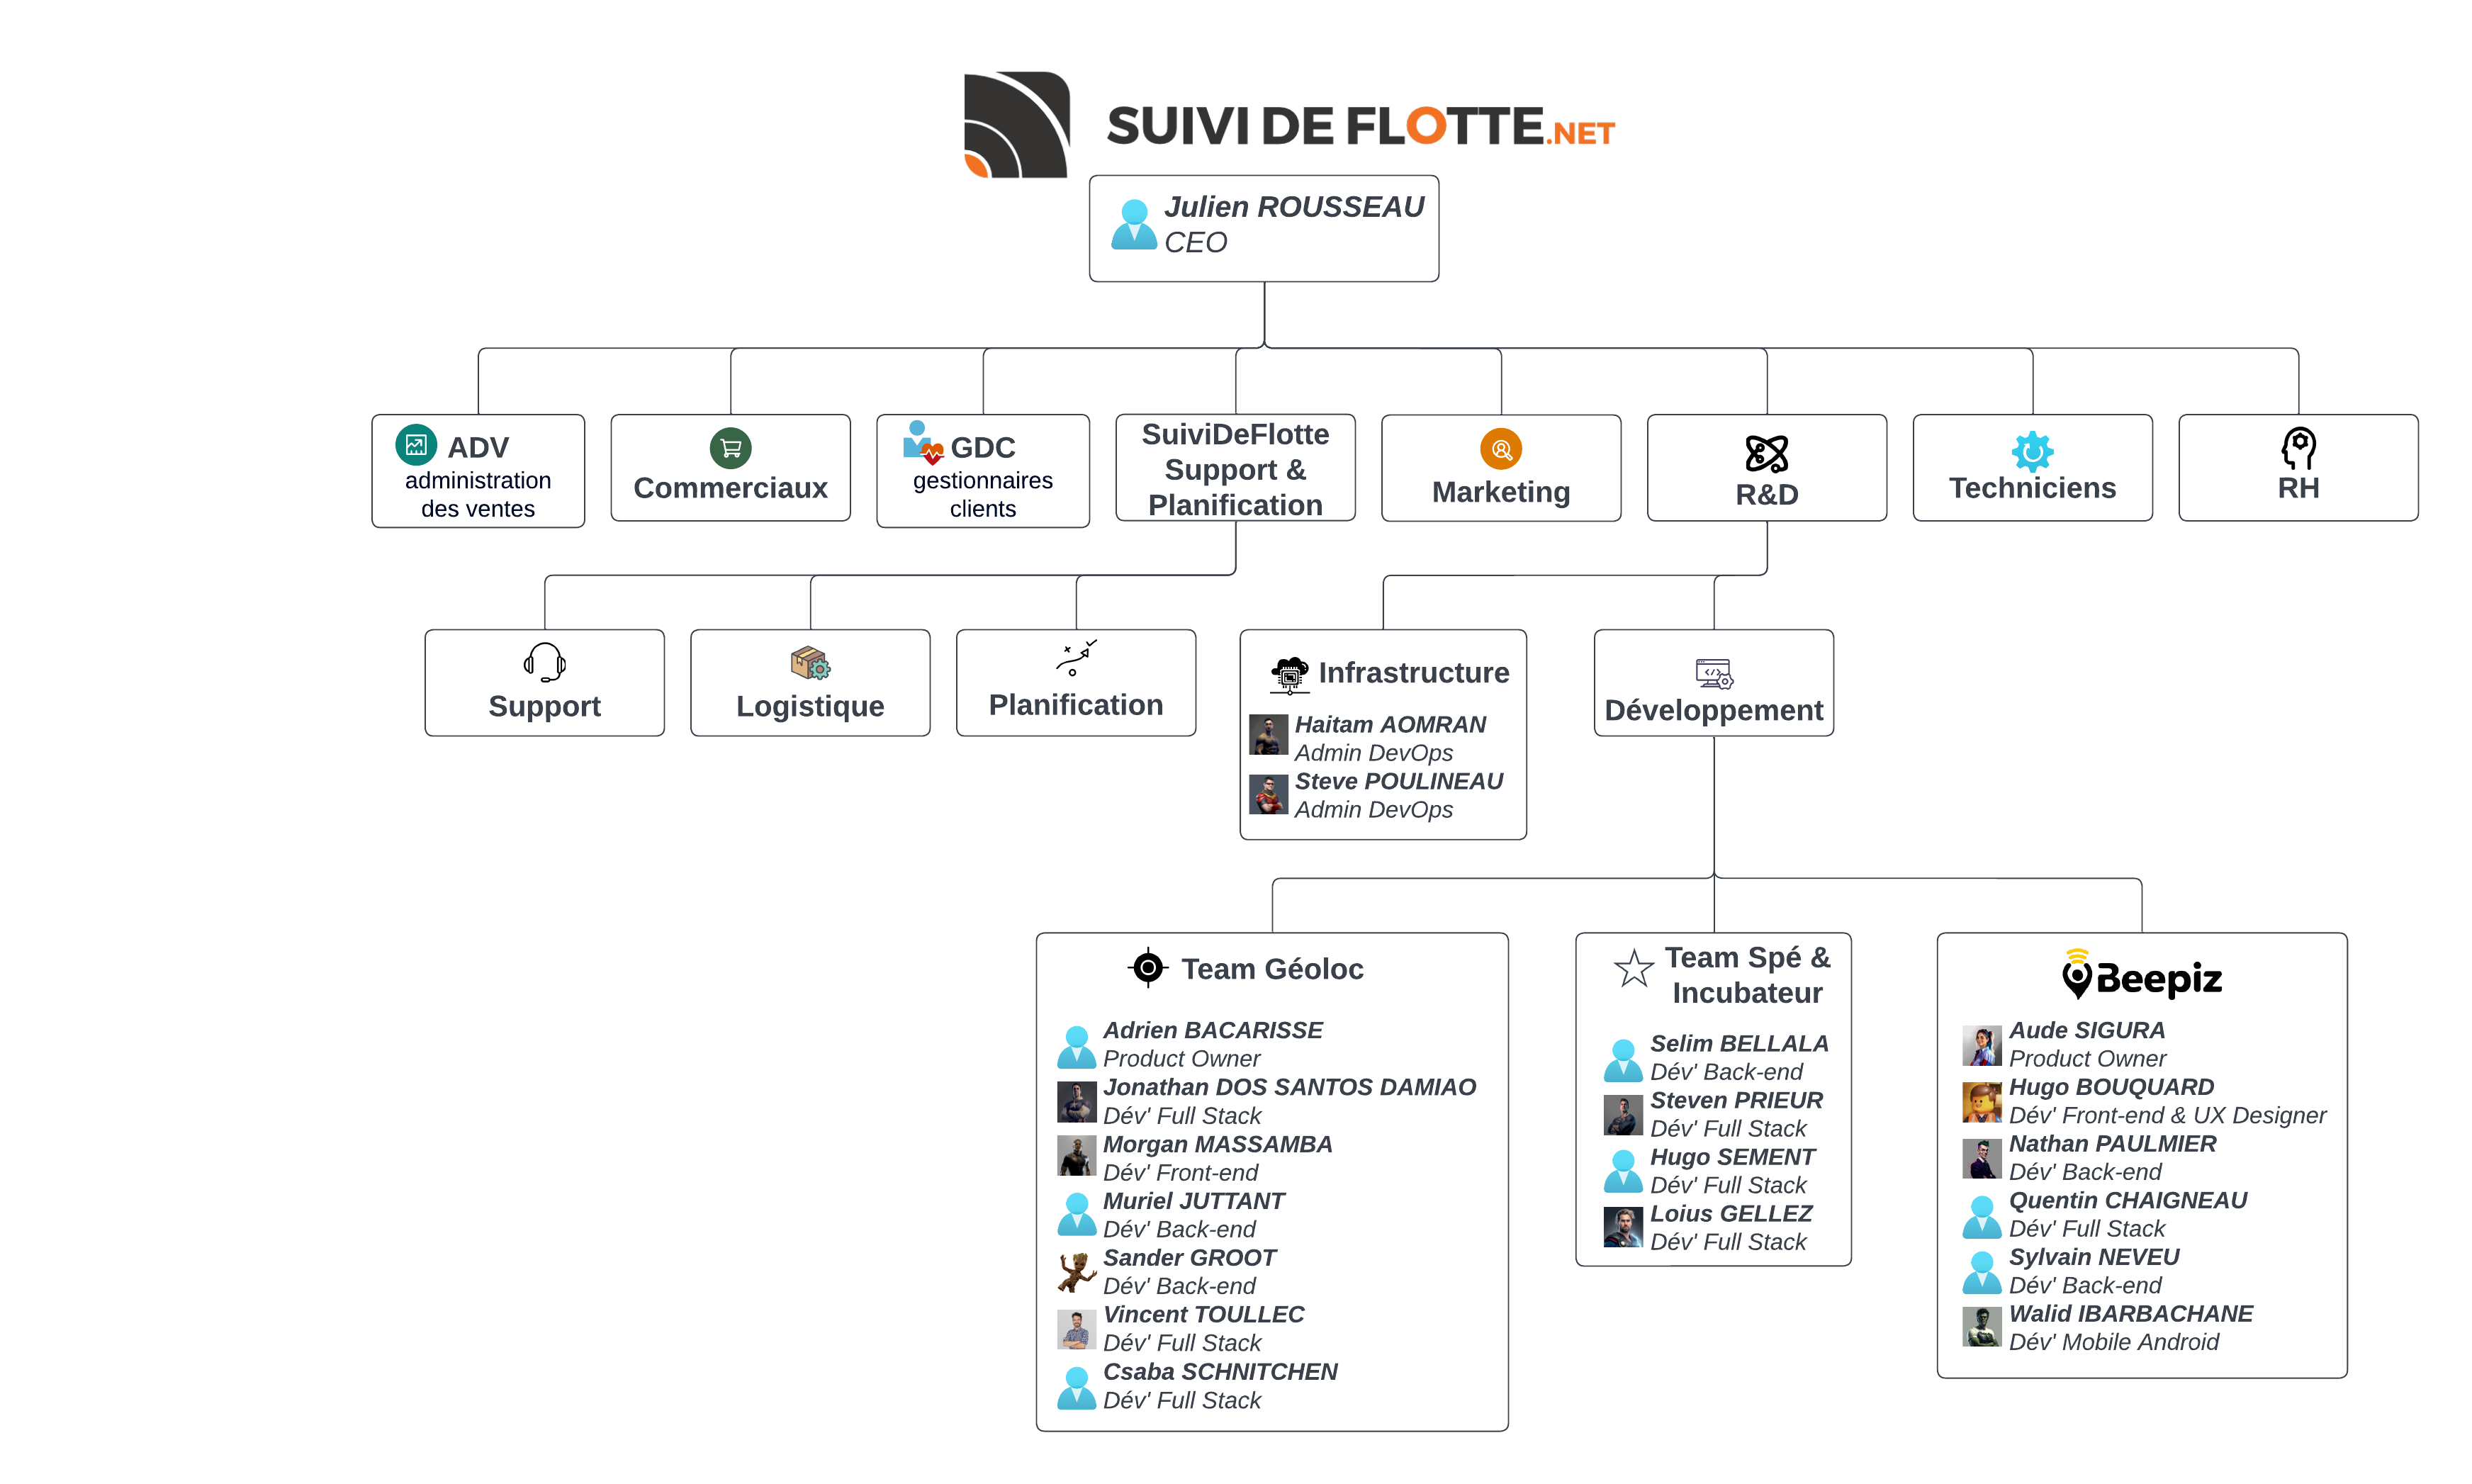
\includegraphics[width=\textwidth]{img/organogram}
    \caption{Organigramme}
    \label{fig:organogram}
\end{sidewaysfigure}

\subsection{La petite histoire de SuiviDeFlotte.net}\label{subsec:histoire-sdf}

SuiviDeFlotte.net, créée en 2001, est la branche de l'entreprise spécialisée dans la géolocalisation et la gestion de flottes de véhicules et d'objets connectés pour les entreprises. À l'origine de cette initiative se trouve Julien Rousseau, actuel Président Directeur Général, qui a remarqué que la gestion de la flotte automobile était le deuxième poste de dépense le plus important pour les entreprises. Pour optimiser ces parcs automobiles et améliorer la productivité des métiers nécessitant des interventions sur le terrain, il a envisagé d'appliquer les succès de la télécommunication aux véhicules.

Les bénéfices potentiels de la télématique embarquée se sont avérés concluants, conduisant ainsi à la création officielle de SuiviDeFlotte.net, pionnière de la télématique embarquée en France. Initialement centrée sur la géolocalisation des véhicules, l'entreprise a progressivement élargi ses services pour offrir des outils complets de gestion de flottes, incluant la géolocalisation, la gestion de parc et l'éco-conduite. Depuis ses débuts, SuiviDeFlotte.net propose ses services via une plateforme SaaS, permettant d'ajouter de nouvelles fonctionnalités aux utilisateurs sans installation ni maintenance.

Aujourd'hui, l'entreprise se focalise sur l'innovation, cherchant à répondre aux besoins de ses utilisateurs en proposant trois grandes mises à jour par an, intégrant plus de 100 nouvelles fonctionnalités chaque année. SuiviDeFlotte.net conçoit et commercialise des solutions clés en main de géolocalisation, écoconduite et gestion de flottes de véhicules (VL, VU, poids lourds), qui sont utilisées par 4000 entreprises, qu'il s'agisse de TPE, PME ou entités de grands groupes. Elle compte 50 collaborateurs, génère un chiffre d'affaires de 7 millions d'euros et consacre 25\% de son effectif à la recherche et développement.